\section{Overview of the AMR}
The general schema of any Adaptive Mesh Refinement algorithm is described in the algorithm \Cref{algorithm:AMRGen}:
\ \\
\begin{algorithm}[H]
 \KwData{Mesh $T_0$}
 \KwResult{A mesh $T_n$ and a solution $\bfy_n$ on this mesh satisfying the solution acceptance criteria}
 i = 0\\
 \While{true}{
  obtain solution $\bfy_i$ on $T_i$\\
	evaluate solution $\bfy_i$ acceptance criteria\\
	\eIf{solution acceptance criteria satisfied} {
		return\\
   } {
		identify subset $T^{r}_i$ of all elements $K \in T_i$ to be refined, $T^{r}_i \subseteq T_i$\\
		obtain $T_{i+1}$ by refining (at least) all $K \in T^{r}_i$\\
		i = i + 1\\
	}
 }
 \caption{Generic AMR algorithm}
\label{algorithm:AMRGen}
\end{algorithm}
In \Cref{algorithm:AMRGen}, \textit{solution acceptance criteria} is usually either spatial error estimate threshold, or number of elements, etc. In the same description, the note that there might be other elements $K \notin T^{r}_i$ refined in order to maintain some desired attributes of the mesh, such as 1-irregularity (the refinement level difference of two elements sharing a common face is at most one), smoothness of mesh (there is e.g. no unrefined elements for which all, or a majority of neighboring elements would be refined), etc.
An example of several steps of the algorithm (where step number corresponds to the variable $i$ in \Cref{algorithm:AMRGen}, is given in \Cref{figure:amrsimple} below on a sample problem in 2 dimensions.

\begin{figure}[H]
	\begin{subfigure}[H]{40mm}
					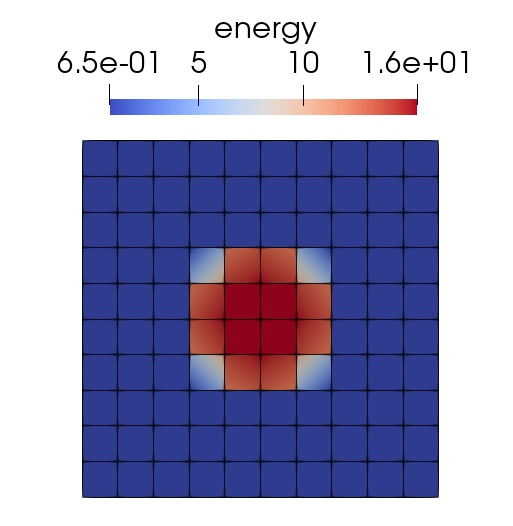
\includegraphics[width=\textwidth]{img/adapt/sln0.jpg}
					\caption{AMR step 0 - 100 elements}
	\end{subfigure}
	\hspace{7mm}
	\begin{subfigure}[H]{40mm}
					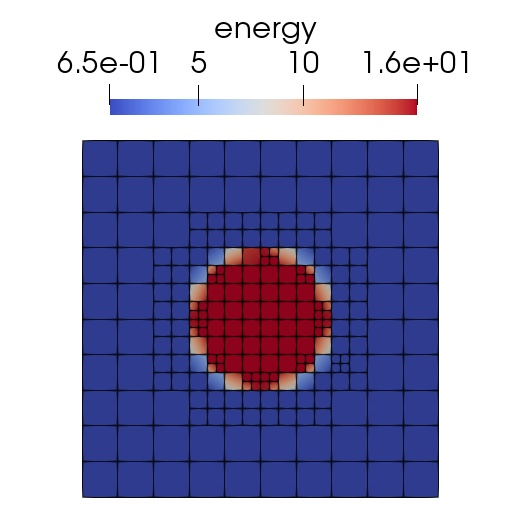
\includegraphics[width=\textwidth]{img/adapt/sln1.jpg}
					\caption{AMR step 1 - 232 elements}
	\end{subfigure}
	\hspace{7mm}
	\begin{subfigure}[H]{40mm}
					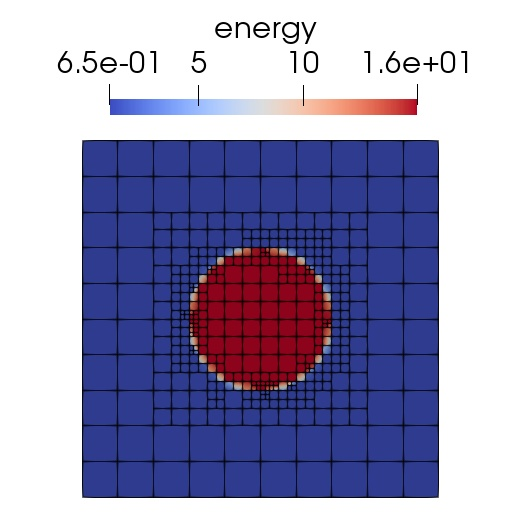
\includegraphics[width=\textwidth]{img/adapt/sln2.jpg}
					\caption{AMR step 2 - 379 elements}
	\end{subfigure}
	\\
	\begin{subfigure}[H]{40mm}
					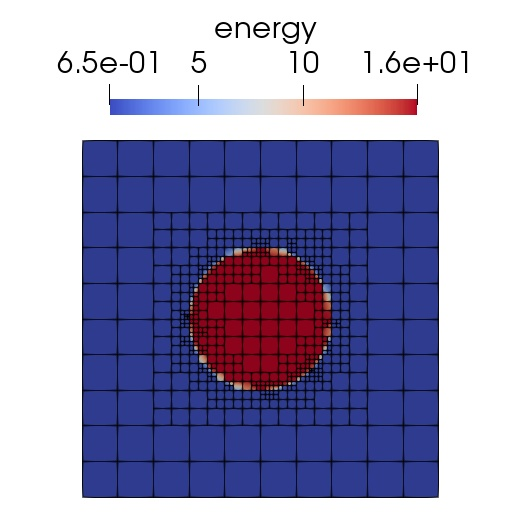
\includegraphics[width=\textwidth]{img/adapt/sln3.jpg}
					\caption{AMR step 3 - 610 elements}
	\end{subfigure}
	\hspace{7mm}
	\begin{subfigure}[H]{40mm}
					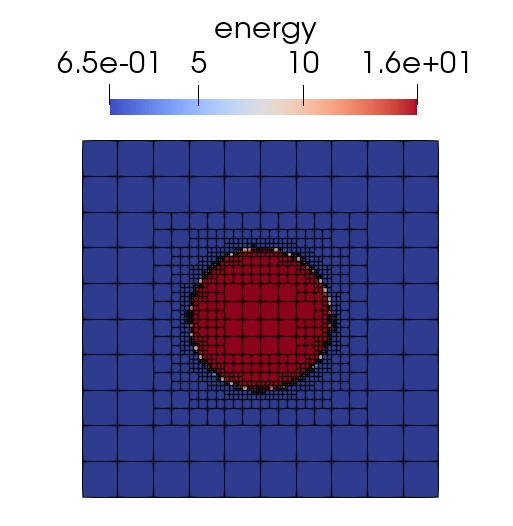
\includegraphics[width=\textwidth]{img/adapt/sln4.jpg}
					\caption{AMR step 4 - 1016 elements}
	\end{subfigure}
	\hspace{7mm}
	\begin{subfigure}[H]{40mm}
					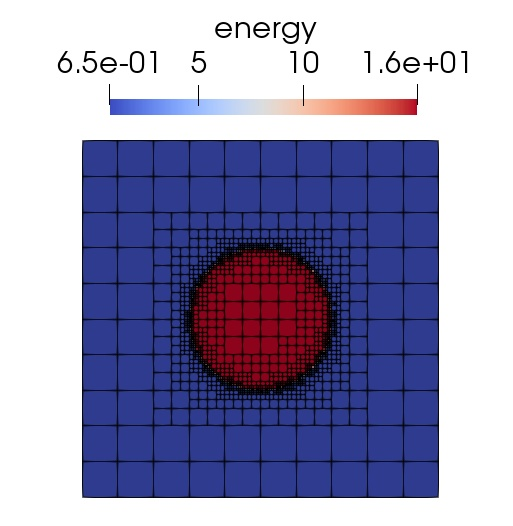
\includegraphics[width=\textwidth]{img/adapt/sln5.jpg}
					\caption{AMR step 5 - 1364 elements}
	\end{subfigure}
		\vspace{3mm}
	\caption{AMR steps}
	\label{figure:amrsimple}
\end{figure}

The benefit of AMR is clear. If we were to discretize the entire domain with elements small enough to capture the solution with the same quality as in the last AMR step, we would end up with $> 40000$ elements, where with AMR, the same is achieved with $< 1400$.

\paragraph{}
Since we are dealing with evolution equations, it is necessary to specify how the AMR algorithm relates with the non-AMR solution algorithm \Cref{algorithm:timeStepping}. There are several points we need to take into considerations:
\begin{itemize}
	\item slope limiting as a postprocessing step after the solution must not be omitted in case of higher-order (e.g. linear) basis functions
	\item the solution needs to be transferred to the refined mesh in order to be able to assemble the matrix and the right-hand side on the refined mesh in the next adaptivity iteration
	\item since the solution evolves and the refinements that contribute to error reduction at time step $n$ do not contribute to error reduction at time step $n + m$ (the solution was e.g. oscillating or potentially discontinuous at time step $n$, but is smooth at time step $n + m$), we also want to revert such refinements as the simulation time progresses, we call this process \textit{coarsening} of elements. For this we shall define a set $T^{c}_i$ of all elements to be coarsened.
\end{itemize}
The algorithm looks like this:

\begin{algorithm}[H]
\textbf{    Set: }$y_0 =\ $ (initial solution)\\
\textbf{    Set: }$ts = 1 $ \# initial time step\\
\textbf{    Set: }$t = 0.00 $ \# initial time\\
    \# Loop over time steps\\
    \For{$;\ t < T;\ t = t+\tau,\ ts = ts + 1$}{
			\KwData{Solution from the previous time step $y^{ts - 1}$ expressed on the mesh $T^{ts}_0$}
			 i = 0\\
			 \While{true}{
				call procedure \Cref{algorithm:singleTimeStep} to obtain $A_{i}, b_{i}\lo y^{ts - 1}_{i}\ro$ on the mesh $T^{ts}_i$\\
				solve the problem $A_i y^{ts}_i = b_{i}\lo y^{ts - 1}_i\ro$\\
				post-process the solution $y^{ts}_i$ using \Cref{algorithm:limiter}\\
				evaluate solution $y^{ts}_i$ acceptance criteria\\
				\eIf{solution acceptance criteria satisfied} {
					$y^{ts} = y^{ts}_i$\\
					break While loop\\
				 } {
					identify subset $T^{r}_i$ of all elements $K \in T^{ts}_i$ to be refined, $T^{r}_i \subseteq T^{ts}_i$\\
					identify subset $T^{c}_i$ of all elements $K \in T^{ts}_i$ to be coarsened, $T^{c}_i \subseteq T^{ts}_i$\\
					obtain $T^{ts}_{i+1}$ by refining (at least) all $K \in T^{r}_i$ and coarsening a subset of $T^{c}_i$\\
					transfer the solution $y^{ts}_i$ onto $T^{ts}_{i+1}$\\
					i = i + 1\\
				}
		 }
			calculate updated value of $\tau$ using \Cref{equation:CFLcond}\\
	 }
\caption{AMR for time-discretized problems}
\label{algorithm:AMRFull}
\end{algorithm}

TODO - tady time dep.

The critical points of the algorithm \Cref{algorithm:AMRFull}are
\begin{itemize}
\item solution acceptance criteria evaluation,
\item identification of subset $T^{r}_i$,
\item identification of subset $T^{c}_i$.
\end{itemize}
For the last two points, we shall consider a function $r$
\be
\label{refinementIndicator}
r:\ T^{ts}_i \rightarrow [0, +\infty),
\ee
which shall be called \textit{refinement indicator}, and the set $T^{r}_i = \left\{K^{r}\right\}$ shall be then defined as a set of all such elements for which one of these criteria are satisfied:
\begin{itemize}
	\item $r\lo K^{r}\ro > \alpha \cdot \max\left\{r\lo K\ro\ |\ K \in T^{ts}_i\right\}$, or
	\item $r\lo K^{r}\ro > \beta \cdot \sum\left\{r\lo K\ro\ |\ K \in T^{ts}_i\right\}$.
\end{itemize}

The set $T^{c}_i = \left\{K^{c}\right\}$ shall be defined similarly as
\begin{itemize}
	\item $r\lo K^{c}\ro < \gamma \cdot \max\left\{r\lo K\ro\ |\ K \in T^{ts}_i\right\}$, or
	\item $r\lo K^{c}\ro < \delta \cdot \sum\left\{r\lo K\ro\ |\ K \in T^{ts}_i\right\}$.
\end{itemize}

Note that the parameters $0 < \gamma \leq \alpha < 1,\ 0 < \delta \leq \beta < 1$ are artificial, and do not affect the overall solution quality (as the solution acceptance criteria has to be met independently of choices of their values). Nevertheless, the choices may affect performance - e.g. for a high $\alpha, \beta$, many steps are needed in order to satisfy the solution acceptance criteria, and on the other hand, if values are too low, there is an unnecessary high number of degrees of freedom that do not contribute substantially to the reduction of the solution error.
\paragraph{}
Please also note, that description of edge cases, and limitations are not given here for brevity. These cases include e.g. what happens if an element is both selected for coarsening and refinement, or how we maintain a 'minimal' refinement level so that we do not coarsen beyond a rational limit.